\documentclass[10pt,aspectratio=169]{beamer}


  \usetheme{NYU}      % or try Darmstadt, Madrid, Warsaw, ...
  \usecolortheme{default} % or try albatross, beaver, crane, ...
  \usefonttheme{default}  % or try serif, structurebold, ...
  \setbeamertemplate{navigation symbols}{}
  \setbeamertemplate{caption}[numbered]
\usepackage{appendixnumberbeamer}
\usepackage{mymacro}


\newcommand{\ind}{\perp\!\!\!\!\perp} 
\usepackage{hyperref}
\usepackage{minted}
\usepackage[round]{natbib}

\hypersetup{
    colorlinks=blue,
    linkcolor=blue,
    filecolor=blue,      
    urlcolor=blue,
    citecolor=blue,
}

% If you want to print handouts
%\documentclass[handout]{beamer}

% Changing the fonts: this will make the slides more readable and the math look like regular tex math
%\usefonttheme{arial}

% Titles will appear in Small Cap Serif



% -----------------------------------------
% Center the Frame Title
% -----------------------------------------




% -----------------------------------------
% Number the slides
% -----------------------------------------

\setbeamertemplate{footline}[frame number]

% -----------------------------------------
% Get rid of the irritating navigation bar
% -----------------------------------------

\setbeamertemplate{navigation symbols}{}
% -----------------------------------------
% Begin Document
% -----------------------------------------
\title{\Large\textsc{The 4T Will Not Be Televised, It Will Be Livestreamed: Censorship and Narrative Control in Mexico}}
\author[Zago] % Esto es lo que sale en el footer
{\textbf{Eduardo Zago}\inst{1}  \vspace{10pt}}

\institute []% Esto es lo que sale en el footer
{  \inst{1}   PhD Student NYU Politics}

\date{\textsc{}}

\titlegraphic{\hfill\includegraphics[height=1.5cm]{nyu_stacked_color}}


\begin{document}
\maketitle
%  I separate each slide with a line:

% -----------------------------------------

%  I start with the screen black, like using the b key in Powerpoint



% -----------------------------------------
%  Restore normal white background

\beamersetaveragebackground{white}


% -----------------------------------------

%  Example of a slide with animated math:
\section{Motivation}


\begin{frame}{Why Governments Hold Interactions with Media?}
\begin{itemize}
  \setlength\itemsep{1em}

    \item Globally, governments increasingly trying to speak \alert{directly} to audiences and to \alert{manage press access} through controlled formats (press pools, livestreams, social media).
    \item President Trump has had more exchanges with the press than 6 predecessors {\footnotesize\color{gray}\citep{Trump100Days}}. 
    \item Also, Andres Manuel Lopez Obrador (AMLO), ex-president of Mexico held 1,423 2-hour press conferences during his tenure.
    \item \textbf{Broadly, I would like to shed some light on what are the incentives (and costs) of both, the government and the media, to have these recurrent interactions?}

    
\end{itemize}
\end{frame}

%%%%%%%%%%%%%%%%%%%%%%%%%%%%%%%%%%%%%%%

\section{Background}


\begin{frame}{Why Governments Hold Interactions with Media?}
\begin{itemize}
  \setlength\itemsep{1em}


  \item Following his 2018 victory, President L\'opez Obrador (AMLO) created a direct-to-public communication channel: the \textbf{\textit{Mañanera}}.

  \item The \textit{Mañanera} is a daily agenda-setting press conference where access to the microphone depends heavily on \textbf{visibility and physical proximity} (front rows).

  \item Initially, a ``first-come, first-served'' rule generated \textbf{adverse selection of questioners}: front-row access became concentrated among aligned outlets, limiting critical questioning and undermining perceived credibility (or anecdotal evidence seem to suggest \citep{Tombola-Razon})

  \item In April 2022, the administration introduced a \alert{daily seat lottery} for the first three rows to broaden access and restore engagement.
\end{itemize}
\end{frame}

%%%%%%%%%%%%%%%%%%%%%%%%%%%%%%%%%%%%%%%%

\begin{frame}
    \begin{figure}
        \centering
        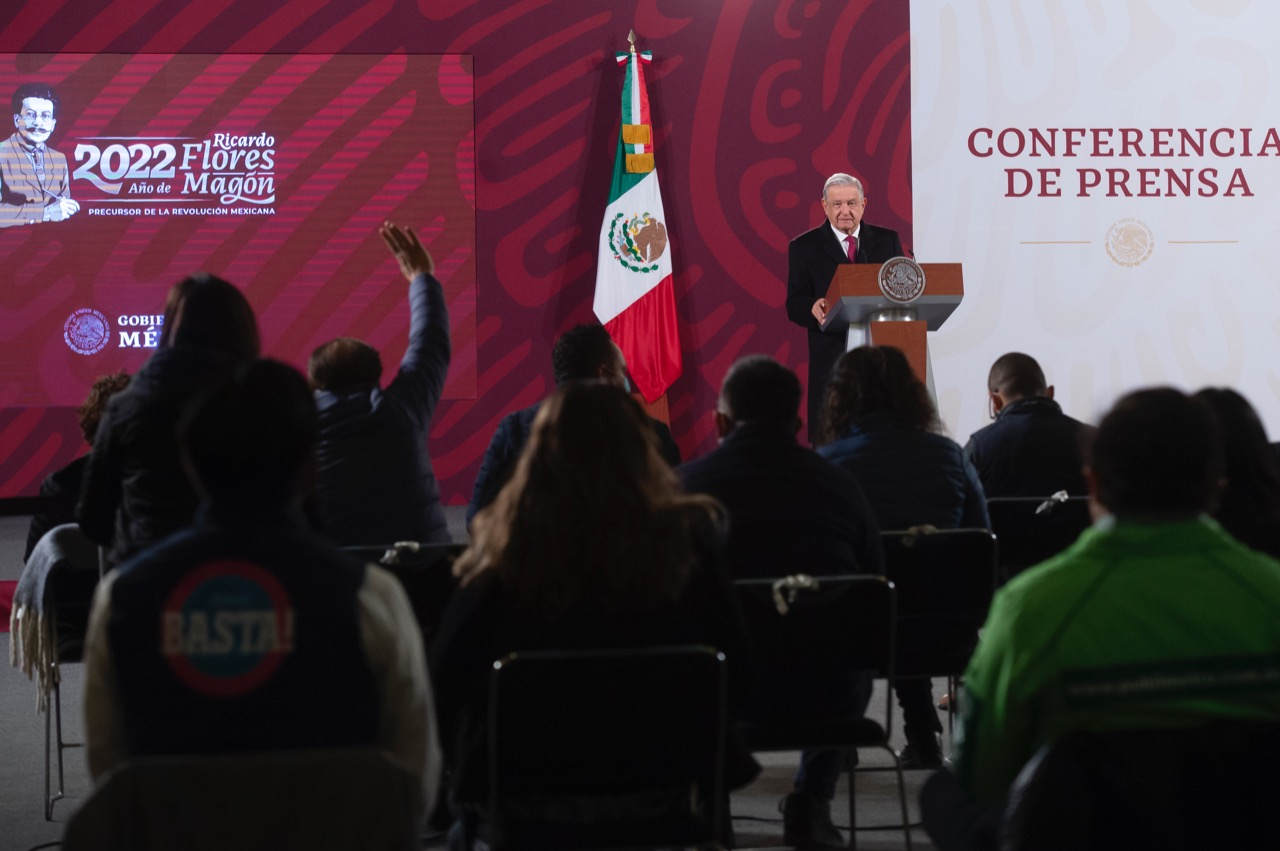
\includegraphics[width=.8\textwidth]{figures/descriptive_stats/mañanera_ex.jpeg}
        \vspace{-0.2cm}
        \caption{\scriptsize Example of a Mañanera}
    \end{figure}
\end{frame}

\section{Why this is important?}

% --- First slide in section: Why this is important? ----------------------------

\begin{frame}
\frametitle{Repeated Media Government Interactions in Democracies}

\begin{itemize}
 \item \textbf{Assuming, even in democracies, governments would like favorable coverage:}
    Direct repression is costly and often constrained, but government still has techniques to silence critics {\footnotesize\color{gray}\citep{Censor-Pratt-AER}}.
    \vspace{0.2cm}
\item Which instruments are used?

\begin{enumerate}
    \item \textbf{Bribery:} Montesinos in Peru {\footnotesize\color{gray}\citep{Peru-Macmillan-JEP}}.
    \item \textbf{De-legitimization:} South Korea \textit{giraegi} and Trump in US {\footnotesize\color{gray}\citep{KoreaJour-Shin-Journalism, PressCriticism-Carlson-Journalism}}.
    \item \textbf{Restriction of source access:} Kisha clubs in Japan {\footnotesize\color{gray}\citep{Kisha-Freedom}}.
    \item \textbf{Public resource allocation:} Argentina and Hungary governments use \alert{advertising} to \alert{reward} supportive outlets and \alert{discipline} critics {\footnotesize\color{gray}\citep{ArgCorr-DiTella-AEJAE, MediaCaptures-Zeidl-Econometrica}}.
\end{enumerate}

\vspace{0.2cm}
\item \textbf{How effective are they?}
\begin{itemize}
  \item \alert{Not Clear!} We rarely observe clean exogenous variation in exposure to dissent and government responses, causal identification is rare for most of these.
\end{itemize}
\end{itemize}
\end{frame}

\begin{frame}{What this paper adds (Cont.)}
\begin{itemize}\setlength\itemsep{0.85em}

\item \textbf{Why the literature gets stuck:}
  \begin{itemize}\setlength\itemsep{0.25em}
    \item \textbf{Dissent is usually endogenous:} aligned outlets self-select into access and favorable treatment
    {\footnotesize\color{gray}\citep{ArgCorr-DiTella-AEJAE}}.
    \item \textbf{Credible commitment is hard to observe:} we rarely see reforms that plausibly change
    \textit{who can speak} and \textit{how they are rewarded} in a way that can be brought to the data.
    \item \textbf{Credibility is hard to measure:} we rarely observe clean proxies for audience attention in government messaging
    {\footnotesize\color{gray}\citep{PersuasionEmpirical-Dellavigna-AR}}.
  \end{itemize}
  
  \item \textbf{What my setting lets me do:}
  A daily seat lottery provides quasi-random variation in \alert{access to the mic},
  and rich administrative data let me trace its consequences.
\end{itemize}
\end{frame}

\section{Context}

\begin{frame}{How the Seat Lottery Works}
\begin{itemize}
  \setlength\itemsep{0.8em}

  \item After April 2022, access to the \alert{first three rows} started depending on \alert{daily lottery} among accredited attendees.

  \item The lottery is \alert{stratified by media type}: seats are drawn separately within categories (e.g., print, TV, radio, digital), and then assigned to the front rows.

  \item Rotation rule: outlets that asked a question the day before are excluded from the lottery.

  \item My identifying claim is simple: \alert{within day $\times$ media type $\times$ not-asked-yesterday}, who lands in the first rows is as-good-as random.
\end{itemize}
\end{frame}

\begin{frame}{Relevance: lottery shifts who gets the mic and what gets aired}
\small
\begin{itemize}\setlength\itemsep{0.65em}

  \item \textbf{Seat location predicts voice.}
  In a hand-coded sample of 10 randomly selected conferences, the distribution of questions by row is:
  \[
  \text{Row 1: }71\% \quad\text{Row 2: }20\% \quad\text{Row 3: }4.5\% \quad\text{Other: }4.5\%.
  \]

  \item \textbf{Implication: it shifts the on-air ``question market.''}
  If being in the first rows is the main bottleneck, randomizing those seats should:
  \begin{itemize}\setlength\itemsep{0.35em}
    \item \alert{deconcentrate} question access (fewer outlets monopolizing the mic), and
    \item increase the probability that \alert{more critical outlets} are the ones whose questions become salient on air.
  \end{itemize}

  \item \textbf{What this buys me empirically:}
  lottery-induced variation in \emph{who} gets front-row visibility generates quasi-random variation in \emph{who} gets to ask, conditional on attending.

\end{itemize}
\end{frame}

\section{Data}

\begin{frame}{Data: What I have, What I can get}
\small
\textbf{I have:}
\begin{itemize}\setlength\itemsep{0.35em}
    \item \textbf{Youtube viewership and Google Trends}: proxy for private advertising benefits of media companies 
    \item \textbf{Government advertising} (via COMSOC contracts): public benefits to media companies / censorship/advertising resources from government. 
    
    \item \textbf{Conference transcript:} can infer from this who participated ($P_{it}$), the \alert{dissent} of each participation ($D_{it}$), AMLO's behavior (hostility towards media, amount of time spent talking, etc.)

    \item \textbf{Attendance:} which outlet attended each conference. ($Attend_{it}$)
\end{itemize}
\textbf{I can get}
\begin{itemize}\setlength\itemsep{0.35em}
    \item \textbf{Seat distribution of outlets:} gov't does not have it, working on inferring it from the videos ($Z_{t}$).
    \item \textbf{Approval}: Daily Presidential approval from Mitofsky AMLO Tracking Poll
    \item \textbf{Private advertising}: from Nielsen (far-fetched but looking around)
    \item \textbf{Outlet metadata}: ideology, viewership, etc. 
\end{itemize}
\end{frame}

\section{Empirical Strategy}

\begin{frame}{Reduced Form: Effect of Dissent (IV)}
\small
\begin{itemize}
    \item \textbf{Media Outlet as Unit}: Does dissent lead to more viewership? And therefore more private gains.

\textbf{First stage (relevance):}
\[
\underbrace{ D_{i,t}}_{\text{Level of Dissent}} = \pi \underbrace{ Z_{i,t}}_{\text{1\{First Row\}}} + \lambda \text{Attend}_{it} + X'_{it}\gamma + \alpha_i + \tau_t + \nu_{it}
\]

\textbf{Second stage:}
\[
\underbrace{ Y_{i,t}}_{\text{Media viewership}} = \beta \widehat{D}_{it} + X'_{it}\theta + \alpha_i + \tau_t + \varepsilon_{it}
\]
\end{itemize}

\vspace{0.5em}


\begin{itemize}
    \item \textbf{Conference as Unit}: effects of dissent on AMLO approval, conference viewership, AMLO's strategy
\[
\underbrace{ Y_{t}}_{\text{AMLO Approval}}
\;=\;
\beta\,\underbrace{ \textit{Ratio First Row}_{t}}_{\text{Opp./Total First Row}}
\;+\;
\lambda\,\underbrace{ \textit{Ratio Attendance}_{t}}_{\text{Opp./Total Attending}}
\;+\;
X'_{t}\theta
\;+\;
\varepsilon_{t}
\]
\end{itemize}
\end{frame}

\begin{frame}{Contract Spikes as Allocation Events}
\small
\begin{itemize}\setlength\itemsep{0.7em}
    \item Public advertising contracts are not always assigned smoothly over time.
    
    \item Instead, some institutions assign many contracts on specific dates, often around campaigns, projects, or administrative deadlines.
    
    \item These spikes create high-frequency windows to study whether media outlets change their behavior around contract allocation dates.
    
    \item The goal is to test whether outlets become more aligned, less critical, or more active when contracts are about to be assigned or have just been assigned.
\end{itemize}

\vspace{0.5em}

\end{frame}

\begin{frame}
    \begin{figure}
        \centering
        
\includegraphics[width=\textwidth]{figures/descriptive_stats/top10_daily_contracts_01_imss.pdf}
        \vspace{-0.2cm}
        \caption{\scriptsize}
    \end{figure}
\end{frame}

\begin{frame}
    \begin{figure}
        \centering
        
\includegraphics[width=\textwidth]{figures/descriptive_stats/top10_daily_contracts_07_tren_maya_s_a_de_c_v.pdf}
        \vspace{-0.2cm}
        \caption{\scriptsize}
    \end{figure}
\end{frame}

\begin{frame}{Difference-in-Differences Around Contract Allocation}
\small

\begin{itemize}\setlength\itemsep{0.65em}
    \item I estimate whether interested outlets change their behavior during the period between the campaign call and the contract assignment.
    
    \item The treatment group is composed of outlets likely to compete for campaign \(c\).
    
    \item The control group includes outlets that are unlikely to want that contract, or outlets that do not generally compete for that type of advertising.
\end{itemize}

\vspace{0.4em}

\[
Y_{i,t}
=
\beta
\left(
Interested_{i,c}
\times
StrategicWindow_{c,t}
\right)
+
\alpha_i
+
\tau_t
+
\delta_c
+
X'_{it}\theta
+
\varepsilon_{i,t}
\]

\vspace{0.3em}

\begin{itemize}\setlength\itemsep{0.45em}
    \item \(Y_{i,t}\): dissent, alignment, attendance, tone, or coverage volume.
    \item \(\alpha_i\): outlet fixed effects; \(\tau_t\): date fixed effects; \(\delta_c\): campaign fixed effects.
    \item \(\beta < 0\): interested outlets become less critical during the allocation window.
\end{itemize}

\end{frame}

%%%%%%%%%%%%%%%%%%%%%%%%%%%%%%%%%%%%%%%%%%%%%%%%%%%%%%%%%%%%%


%-----------------------------------------------



\begin{frame}[allowframebreaks]
    \bibliographystyle{apsr}
    \typeout{}

    \singlespacing
    
    \bibliographystyle{apsr}
    \bibliography{biblio}
\end{frame}


\end{document}